\chapter{Componentes básicos en una red}

\section{Router}

\begin{wrapfigure}{r}{0.36\linewidth}
    \centering
    \vspace{-20pt}
    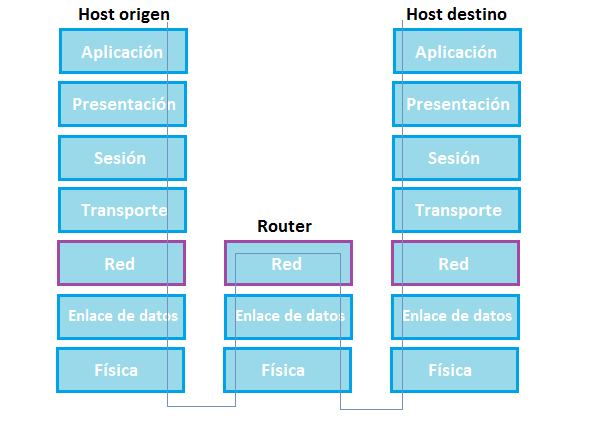
\includegraphics[width=\linewidth]{OSI_model_router.png}
    \vspace{-32pt}
    \captionof{figure}{Router en el modelo OSI (\href{https://es.wikipedia.org/wiki/Router\#/media/Archivo:OSI_model_router.png}{wikipedia})}
    \vspace{-10pt}
\end{wrapfigure}

Un router (o encaminador) es el encargado de enrutar (o encaminar) los paquetes que recibe de una red a otra red buscando la ruta más adecuada para ello.

Un router puede “unir” redes, por lo que para ello es necesario que tenga interfaces configuradas (IPs) en las redes que quiere comunicar. Tendrá tantas interfaces configuradas como redes a las que esté unido.


\begin{center}
    \vspace{-15pt}
    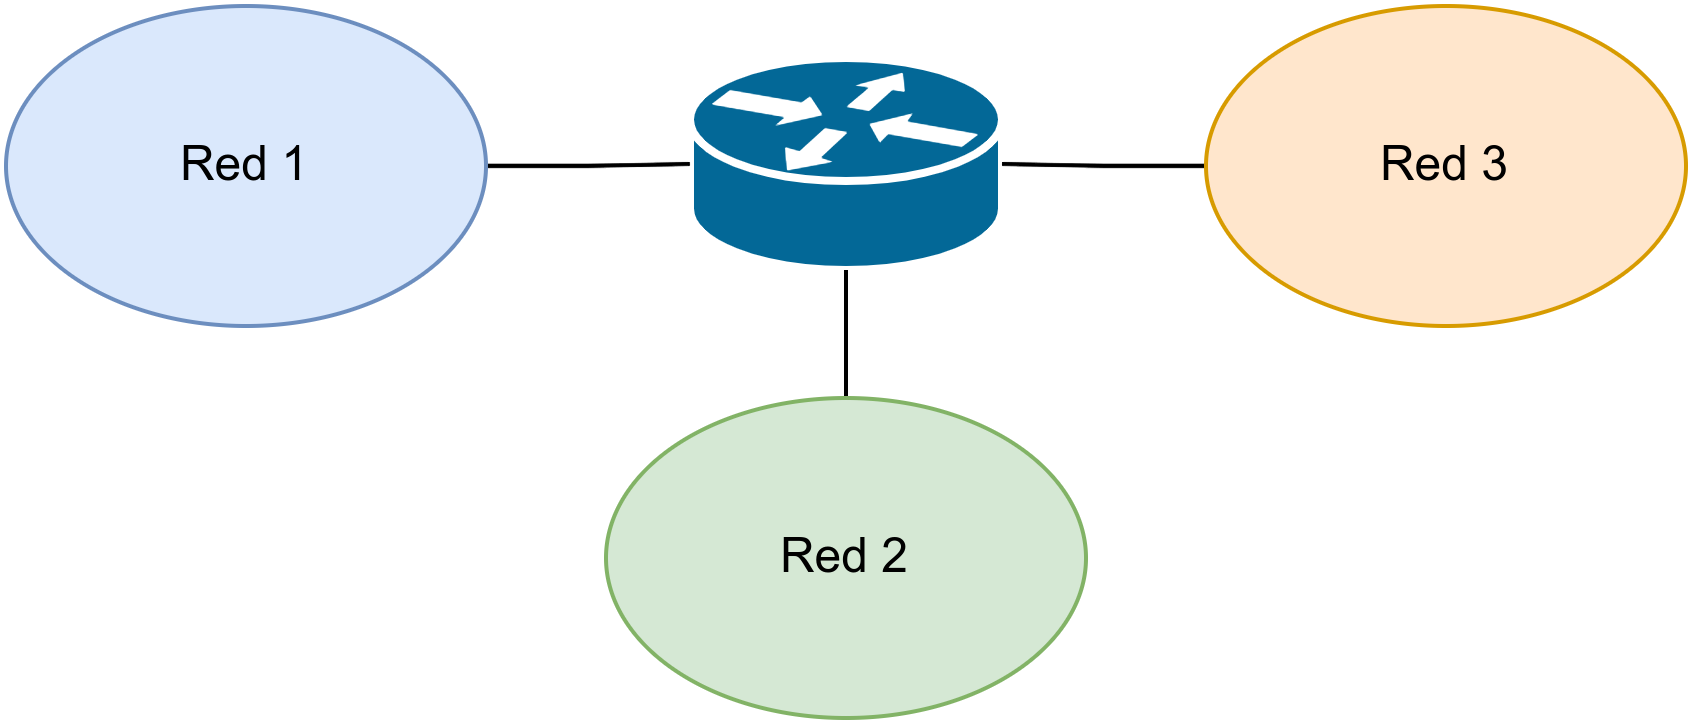
\includegraphics[width=0.6\linewidth]{router_redes.png}
    \vspace{-5pt}
    \captionof{figure}{Router conectado a 3 redes}
    \vspace{-15pt}
\end{center}

El ejemplo más sencillo de router lo tenemos en casa, que es proporcionado por nuestro ISP. Este router une la red privada donde conectamos nuestros equipos (PCs, tablets, móviles) y la red del proveedor que a su vez nos dará acceso a Internet.


\hypertarget{default_gateway}{}
\subsection{Puerta de enlace predeterminada}
La puerta de enlace predeterminada (en inglés \textit{\textbf{default gateway}}) es el dispositivo por defecto por el que irá la comunicación de un equipo cuando trate de comunicarse con una red que no es la suya.

Sin una puerta de enlace, nuestro PC sólo podría comunicarse con otros equipos de la misma red, ya que el switch se encarga de ello, pero no podríamos realizar ninguna comunicación con ningún equipo que estuviese fuera de la red.

\warnbox{\textbf{Los routers también pueden tener puertas de enlace predeterminadas.}}

Los gateway también tienen otras funciones a la hora de intercomunicar redes, como por ejemplo:
\begin{itemize}
    \item Traducir la información que se envía utilizando el protocolo de la red de origen al protocolo utilizado en la red de destino.
    \item Realizar enmascaramiento de la IP de la red origen cambiándola por la IP del dispositivo en la red de destino (también conocido como \hyperlink{nat}{NAT}).
\end{itemize}

Un equipo sólo podrá contar con una puerta de enlace predeterminada configurada, pero mediante \hyperlink{rutas_estaticas}{rutas estáticas} podremos elegir cómo encaminar tráfico a otras redes destino.

\infobox{\textbf{Un equipo sólo podrá contar con una puerta de enlace predeterminada configurada.}}

Para saber cuál es la puerta de enlace de un equipo informático, dependeremos del sistema operativo en el que nos encontremos. En un entorno GNU/Linux actual podremos obtenerlo por consola de la siguiente manera:

\begin{mycode}{Obtener puerta de enlace en GNU/Linux}{console}{}
ruben@ubuntu:~$ ip route
default via 192.168.1.1 dev enp1s0 proto dhcp metric 100
\end{mycode}

En distribuciones antiguas se hacía
\begin{mycode}{Obtener puerta de enlace en GNU/Linux}{console}{}
ruben@ubuntu:~$ route -n

Kernel IP routing table
Destination     Gateway      Genmask      Flags Metric Ref  Use Iface
0.0.0.0      192.168.1.1     0.0.0.0      UG    100    0    0   enp1s0
\end{mycode}


En un entorno Windows, podremos verlo a través del interfaz gráfico yendo a “\textbf{Configuración → Estado de red → Cambiar opciones del adaptador}”, donde veremos los adaptadores que tiene nuestro equipo. Seleccionaremos uno, y haciendo click derecho le daremos a “\textbf{Estado → Detalles}”

\begin{center}
    \vspace{-15pt}
    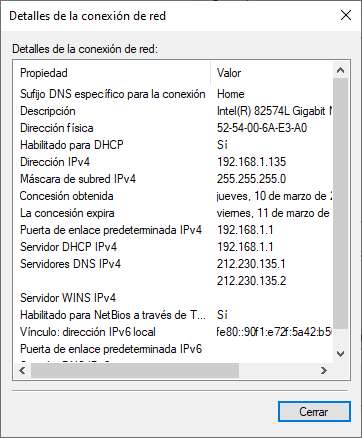
\includegraphics[frame,width=0.4\linewidth]{windows_network_status.png}
    \vspace{-15pt}
\end{center}

Para no dar tantos pasos, si ejecutamos en la terminal \textbf{CMD} el siguiente comando también lo veremos:

\begin{mycode}{Obtener puerta de enlace en Windows}{console}{}
C:\Users\ruben> ipconfig

Configuración IP de Windows
Adaptador de Ethernet Instancia de Ethernet 0 2:

Sufijo DNS específico para la conexión. . : Home
Vínculo: dirección IPv6 local. . . : fe80::90f1:e72f:5a42:b50d%7
Dirección IPv4. . . . . . . . . . . . . . : 192.168.1.135
Máscara de subred . . . . . . . . . . . . : 255.255.255.0
Puerta de enlace predeterminada . . . . . : 192.168.1.1
\end{mycode}

Pueden existir equipos sin puerta de enlace, pero no suele ser lo habitual. Esto sucede cuando queremos que equipos puedan ver a otros equipos de la red, pero no puedan comunicarse con el exterior. Suele ser más habitual realizar bloqueos a nivel de firewall.

\subsection{Router casero}
\begin{wrapfigure}{l}{0.2\linewidth}
    \centering
    \vspace{-20pt}
    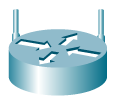
\includegraphics[width=\linewidth]{home_router.png}
    \vspace{-32pt}
\end{wrapfigure}
Los routers caseros son dispositivos que nos permiten conectarnos a internet. El problema es que normalmente suelen ser muy básicos y su funcionalidad es limitada.

Eso no quita que realmente cumpla la función para la que han sido creados, que es la de permitir la interacción de una red como la de un hogar hacia internet.

Los routers caseros suelen tener diferenciada en la parte de atrás el interfaz donde se debe conectar el cable que va hacia Internet (en este caso de color azul) y las bocas que van a formar la red LAN interna de casa (color amarillo), que realmente son un pequeño switch de 4 bocas.

\begin{center}
    \vspace{-15pt}
    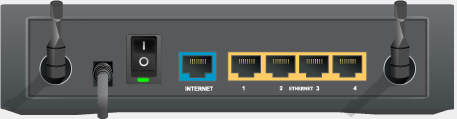
\includegraphics[width=0.7\linewidth]{home_router_back.png}
    \vspace{-4pt}
    \captionof{figure}{Home-Router en Packet Tracer}
    \vspace{-15pt}
\end{center}


Dependiendo del tipo de conexión que tangamos en casa, el interfaz que nos conecta a internet será distinto, pudiendo ser hoy día los más habituales:

\begin{itemize}
    \item \textbf{Cable coaxial}: En conexiones con Euskaltel en el que no nos llega la fibra hasta casa.
    \item \textbf{Conector de fibra}: Cuando la fibra nos llega hasta nuestra casa.
\end{itemize}

Los routers que tenemos en casa también tiene otras funcionalidades básicas que vienen pre-configuradas como veremos a continuación, entre las que podemos destacar:

\begin{itemize}
    \item \textbf{Direccionamiento LAN}: Normalmente viene configurado con la red 192.168.1.0/24 o 192.168.1.0/24

    \item \textbf{\hyperlink{dhcp}{DHCP Server}}: Servicio que otorga IPs en nuestra red LAN, teniendo en cuenta el direccionamiento que tengamos.

    \item \textbf{Configuración Wifi}: Dependiendo del modelo tendremos distintas redes inalámbricas (en distintos rangos). Podremos configurar el nombre de la red, el canal y el tipo de seguridad de acceso a la misma.

    \item \textbf{Restricción hacia internet}: Algunos routers permiten limitar el acceso a Internet en ciertos horarios (ideal para restringir el acceso a menores de edad).

    \item \textbf{Redirección de puertos}: Para redirigir conexiones desde Internet a un equipo concreto dentro de la red.

    \item \textbf{Filtrado MAC}: Normalmente para el apartado Wifi, y así limitar quién se puede o no se puede conectar.
\end{itemize}


\hypertarget{nat}{}
\section{NAT}
La traducción de direcciones de red, también llamado enmascaramiento de IP o NAT (del inglés \textit{\textbf{Network Address Translation}}), es un mecanismo utilizado por routers que conectan dos (o más) redes para que el paquete que llega a un equipo destino no parezca que llega desde la red de origen.

Vamos a tomar como ejemplo el siguiente esquema que es un ejemplo que podemos entender teniendo en cuenta la conexión de nuestra casa:

\begin{center}
    \vspace{-15pt}
    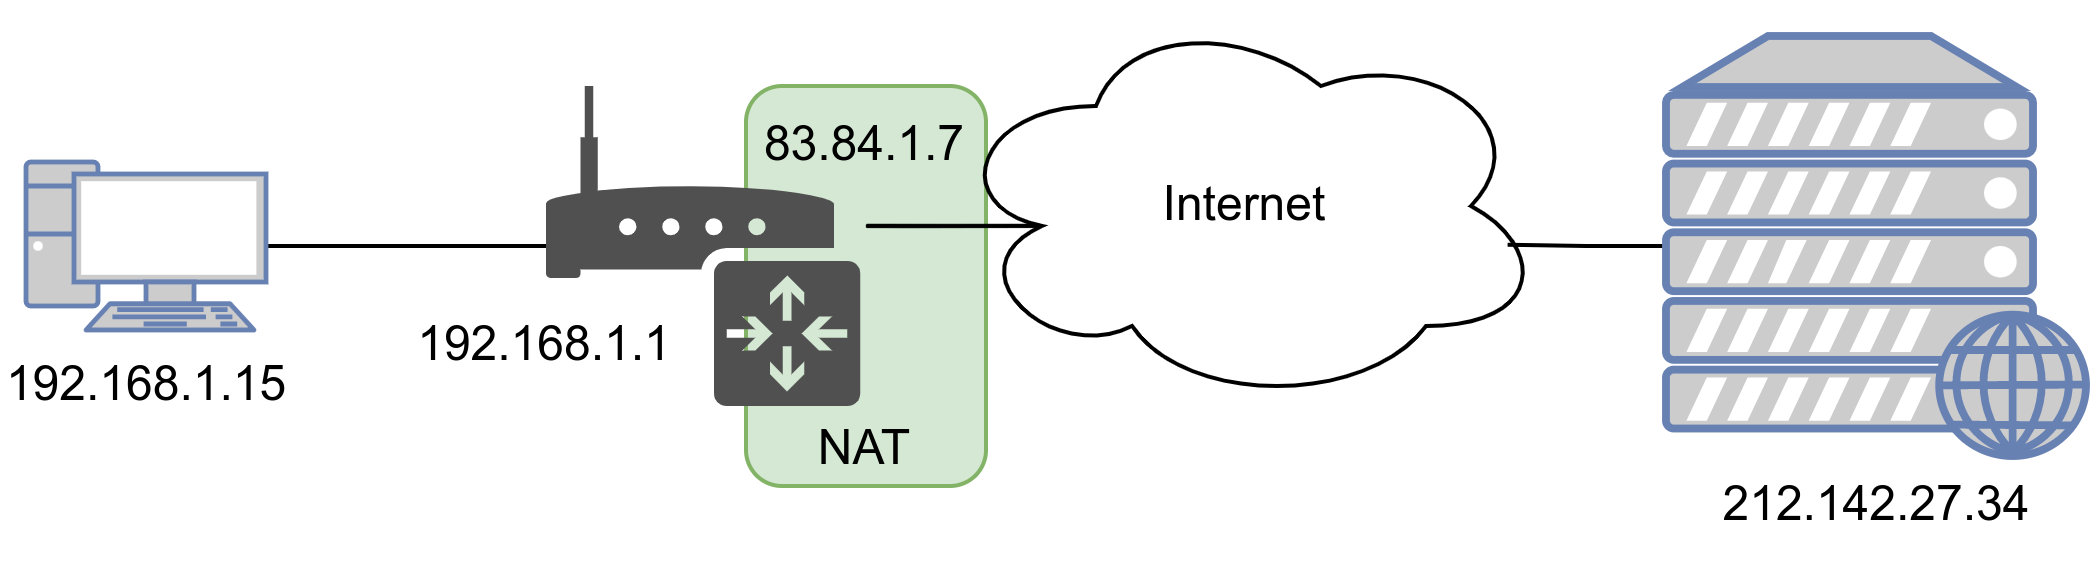
\includegraphics[width=0.8\linewidth]{NAT.png}
    \vspace{-25pt}
\end{center}

En este ejemplo tenemos conectado un equipo con IP 192.168.1.15 al router que tenemos en casa (cuya IP en la LAN es 192.168.1.1). Este router cuenta con una IP pública proporcionada por el ISP para el acceso a internet (83.84.1.7). Cuando nuestro equipo quiere comunicarse con algún equipo que no está en su red, al salir a internet, el router cambia la cabecera del paquete sustituyendo 192.168.1.15 por 83.84.1.7, y de esta manera al servidor remoto (212.142.27.34) el paquete le llega desde una IP pública.

Este es el ejemplo más sencillo y que hacemos uso cada día en casa, pero esto no significa que NAT sólo se realice entre redes públicas y privadas. Lo podemos utilizar entre dos redes públicas o dos redes privadas también.

Las traducciones de dirección se almacenan en una tabla, para recordar qué dirección y puerto le corresponde a cada dispositivo cliente y así saber donde deben regresar los paquetes de respuesta.

Existen distintos tipos de NAT:
\begin{itemize}
    \item \textbf{NAT de sobrecarga}: Varios equipos de la red de origen se traducen por una única dirección de la red de salida. Es el método más habitual (el que realizan nuestros routers en casa).

    \item \textbf{NAT estática}: También conocida como “NAT 1:1”, ya que una dirección IP privada se traduce siempre por una única dirección IP pública, y siempre será la misma. Este método es el habitual cuando queremos tener un servidor en la red interna y queremos que su comunicación con el exterior siempre sea con la misma IP pública

    \item \textbf{NAT dinámica}: Similar al caso anterior, pero en este caso el router contará con una tabla de IPs públicas y se asignará una que esté libre de esta tabla a un equipo interno cuando necesite comunicarse de manera pública. Cuando deje de necesitarlo, la IP se marcará como “libre” y se podrá asignar a otro equipo interno posteriormente.
\end{itemize}

\hypertarget{dhcp}{}
\section{DHCP}
El protocolo de configuración dinámica de host (\textit{Dynamic Host Configuration Protocol}, también conocido por sus siglas de \textbf{DHCP}) es un protocolo de red que nos permite configurar la IP de un dispositivo dentro de una red.

Normalmente el protocolo DHCP enviará la configuración de los siguientes parámetros para que el equipo los use:

\begin{itemize}
    \item \textbf{IP}: IP asignada al equipo.
    \item \textbf{Máscara de red}: para identificar el tamaño de la red.
    \item \textbf{\hyperlink{default_gateway}{Default gateway}}: para que el equipo se pueda comunicar con otra red.
    \item \textbf{DNS}: el servidor DNS que utilizará el equipo para la resolución de nombres.
\end{itemize}

\begin{wrapfigure}{r}{0.2\linewidth}
    \centering
    \vspace{-20pt}
    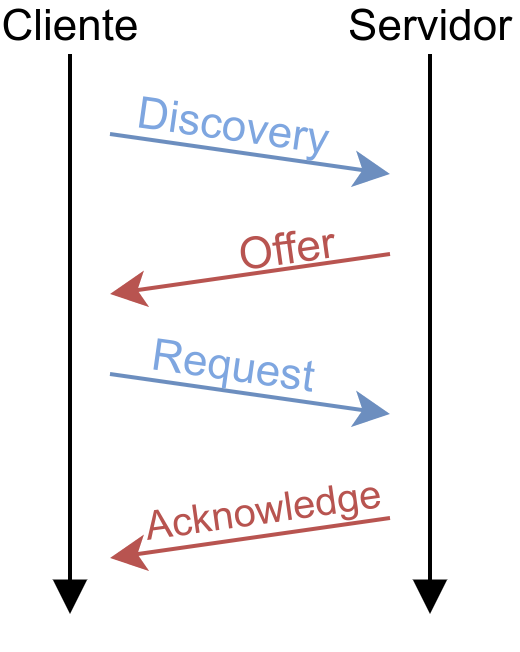
\includegraphics[width=\linewidth]{sesion_DHCP.png}
    \vspace{-32pt}
    \captionof{figure}{\href{https://es.wikipedia.org/wiki/Protocolo\_de\_configuraci\%C3\%B3n\_din\%C3\%A1mica\_de\_host\#DHCP\_Discovery}{Referencia}}
    \vspace{-30pt}
\end{wrapfigure}
Existen muchas más \href{https://es.wikipedia.org/wiki/Par\%C3\%A1metros_DHCP}{configuraciones} que se pueden enviar a un equipo que realiza una petición de configuración por DHCP, pero las arriba expuestas son las más habituales.

El protocolo funciona en forma “Cliente/Servidor”, siendo el equipo el que realiza la búsqueda de un servidor DHCP para el inicio de la configuración. DHCP hace uso de los puertos 67/UDP para el servidor y 68/UDP para los clientes.

Lo más habitual es que el servidor DHCP esté configurado en los routers (tal como sucede en los que nos proporcionan los ISP), pero no tiene por qué ser así, pudiendose instalar en un equipo con Windows Server, GNU/Linux, ...

\subsection{Configuración}
Dependiendo del equipo en el que estemos realizando la configuración del servidor DHCP, el interfaz a configurar podrá ser distinto.